\chapter{Related Work}
\label{chapter_related_work}
In the ever expanding universe of accessible information and the information overload that follows with it, the work on dealing with this overload never sleeps. This chapter will look at work done on handling information overload, especially considering news consumption, and news consumption on mobile devices. Topics like personalization, mobile news applications and news applications in general, designing mobile news applications and information aggregation will be discussed in more detail.

\section{Personalization on mobile devices}

Information handling on regular desktop computers compared to mobile devices comes with different problems, possibilities and focus areas, considering for instance hardware capabilities and area of usage. 

%Mobile devices often have slower network connections, smaller screens and are portable. Therefore the importance of getting the wanted information without too much browsing and network loading is more significant than on a desktop computer where browsing is an easier and cheaper task considering screen size and network connection.

\cite{ricci2010mobile} lists several issues when creating recommender systems for mobile devices:

\begin{itemize}

\item The screen is a lot smaller than on desktop computer resulting in a smaller scrollable area which craves a higher workload from the user to display all the information, which makes the probability of the user seeing all the information smaller.

\item Mobile devices often has limited input and interaction capabilities, which makes the effort of querying higher than on a regular keyboard.

\item Mobile Internet browsing sessions are often shorter than on desktop computers, i.e. in the time span of a couple of minutes.

\item Most web pages are not optimized for mobile devices which may result in a badly formatted displaying of the page.

\item The cost of retrieving the data using mobile data through Edge or 3G are usually much higher than on personal Internet connections at home or office.
\end{itemize}

\section{Personalized news}
\label{related_work_personlized_news}
Personalized news and news applications taking advantage of personalization and recommendation technology is a trending topic now, considering three of the most popular mobile news application has been acquired by major software companies the last couple of months\cite{linkedin_acquires_pulse}\cite{google_acquired_wavii}\cite{summly_sold_yahoo}. Different news personalization approaches has also been researched and proposed the last years.

\cite{billsus2000user} presents a system with focus on design, deployment and evaluation of a client/server-based framework for adaptive news access. Two news agents are described and deployed, one for the web and one on a PDA. The web version uses explicit feedback, and the PDA version uses implicit feedback, and the individual user models based on this feedback are induced by using machine learning algorithms. This feedback are meant to constantly keep the user profile up to date, and empirically build the user profile.

The feedback are translated into short term and long term models, whereas the short term model can propose articles related to stories that has already been read, or not proposing articles similar to ones that already are read. A user can be interested in two different articles concerning a topic, but will most likely not be interested in two similar articles covering the same story although the topic is considered interesting. The long term model can update the user profile's interests with regard to categories the user finds interesting. If the user has read a lot of articles in one specific category over a longer period of time, a safe bet is that this is an interesting category, and can also be added to the user profile as an interesting category.

The framework also proposes a hybrid model where the short term and long term models are combined in such a way that if the short term model cannot classify the feedback, the long term classification is used. 

\begin{figure}[!htbp]
\centering
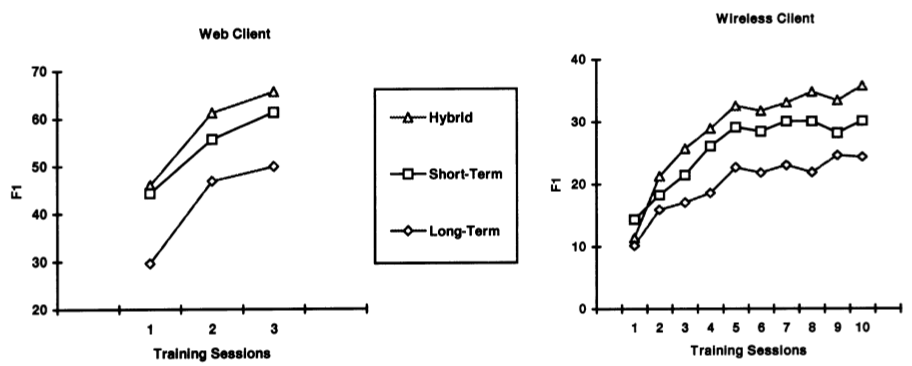
\includegraphics[width=130mm]{GFX/tech/adaptiveNewsAccessShortLongHybridTerm.png}
\caption{The learning curves of the different models used in the adaptive news access framework.}
\label{adaptive_news_access_learning_curves}
\end{figure}

Figure \ref{adaptive_news_access_learning_curves} shows the learning curves of the different models, where F1 is a function to measure the performance of the model. The figure shows that the hybrid approach outperforms both the short term and long term models when used individually. The results of the empirical study of this framework also suggests that effective personalization are obtainable without explicit feedback from the user.




\cite{rohr2008aggregated} proposes a framework for aggregating news articles, extracting the text, images, videos and TV news, turning it into a news event and displaying this in a lucid and clear user interface. The user is then able to select aggregated events based on semantic data, instead of just news articles.

The user interface has three main views, the overview of the different events, the single event view and the tag cloud. The overview shows a list of different events, grouped by date and ordered by their descending score. The single event view show a particular event with corresponding related articles, images, videos and a timeline graph showing the evolution of the event over time in terms of number of resources published per day. The tag cloud is a collection of entities that the personalization engine has set as the user's current topics of interests. The bolder font, the more popular is that particular topic, and the users can remove and add topics as they wish.

\begin{figure}[!htbp]
\centering
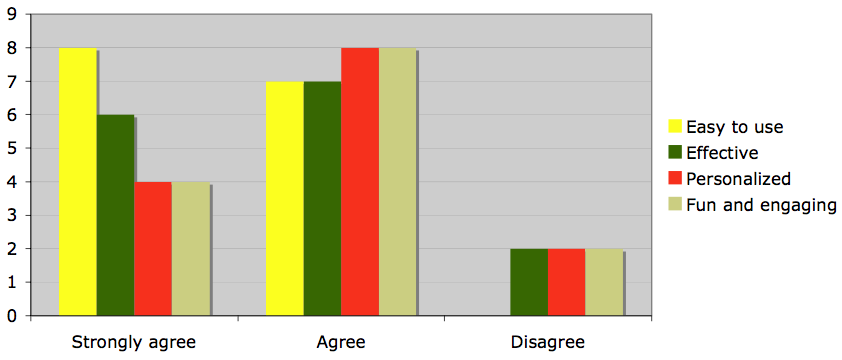
\includegraphics[width=130mm]{GFX/tech/aggregatedExpRating.png}
\caption{Experience rating of the aggregated news system.}
\label{aggregated_news_system_exp_rating}
\end{figure}

The UI allows an easy browsing experience as well as an in-depth understanding of an event. Figure \ref{aggregated_news_system_exp_rating} shows the user feedback of the proposed UI, and it shows that the majority of the users are satisfied with the system.



From the middle of 2007 to late 2010, \cite{thurman2012future} performed a longitudinal study covering how personalization is done at 11 national news websites in the UK and US. Results from the three content surveys conducted in midst 2007, late 2009 and late 2010, showed that there were an increase of 69 per cent in the number of distinct adaptive news categories, from 70 to 118.

\begin{figure}[!htbp]
\centering
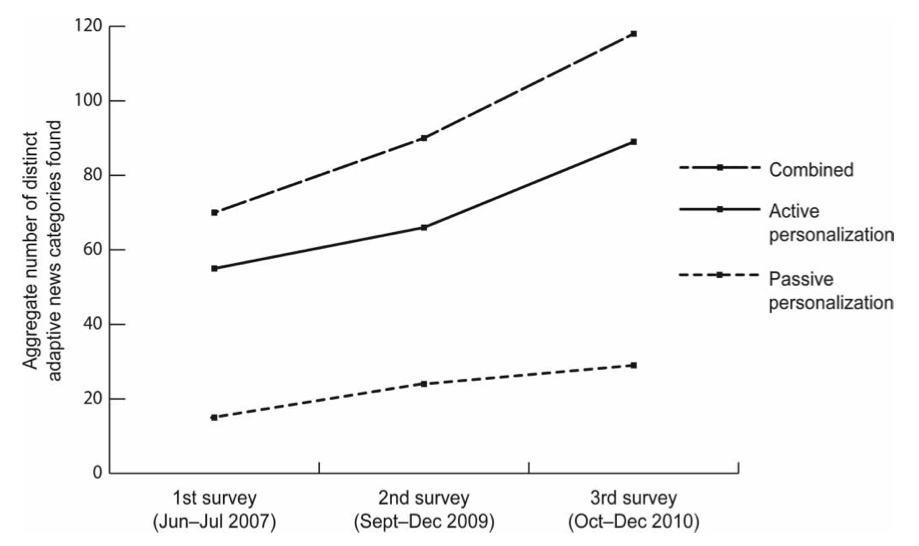
\includegraphics[width=130mm]{GFX/tech/longitudinalStudyIncreaseInPersonalization.png}
\caption{Growth of adaptive news at 11 national US and UK websites, 2007-2010.}
\label{longitudinal_study_increase_in_personalization}
\end{figure}

Another finding was that passive personalization was decreasing while active personalization was increasing, and combined there still was an increase, as shown in figure \ref{longitudinal_study_increase_in_personalization}. It also states that news content providers needs to increase their use of personalization to target advertising better to each specific user, as static advertising is decreasing and dynamic advertising is increasing.

\cite{li2011scene} proposes a scalable two-stage personalized news recommender system, SCENE. The system has two level of news representation, namely the topics relevant to the user preferences and the specific news articles. Further on, the system consists of three main components, clustering of news articles, construction of the user profile and recommendation.

The clustering is done by using probabilistic language models. The user profile construction is done by extracting accessed news content, similar access patterns and preferred name entities from the user's browser log. The recommendation is done by selecting the most similar news group by looking at the clustered news articles and the user profile. Further, from this group, the recommendation is modeled as a "budgeted maximum coverage problem"\cite{khullera1999budgeted} and solved in a greedy way. To finish it up, properties like recency and popularity are taken into account.

SCENE is demonstrated to support high quality recommendation result and an efficient clustering on newly published news articles, through extensive evaluation.


\subsection{Filtering}

\cite{wen2012hybrid} presents a personalized recommendation of news for Web using a hybrid method consisting of both content-based filtering and collaborative filtering. This model provides an autonomous tool that has the ability to minimize tedious and repetitive Web surfing for the user. A classification method, consisting of 5 steps, is used to auto-classify the Web pages. Models representing the user's degree of interest to a specific topic, the user interest model, and the user's preference to use a Web source, the preference model, are created using the Bayes theorem. Also a quantification of the time factor must be done, in addition to the preference model and user interest model, to be able to recommend the news item.

\begin{figure}[!htbp]
\centering
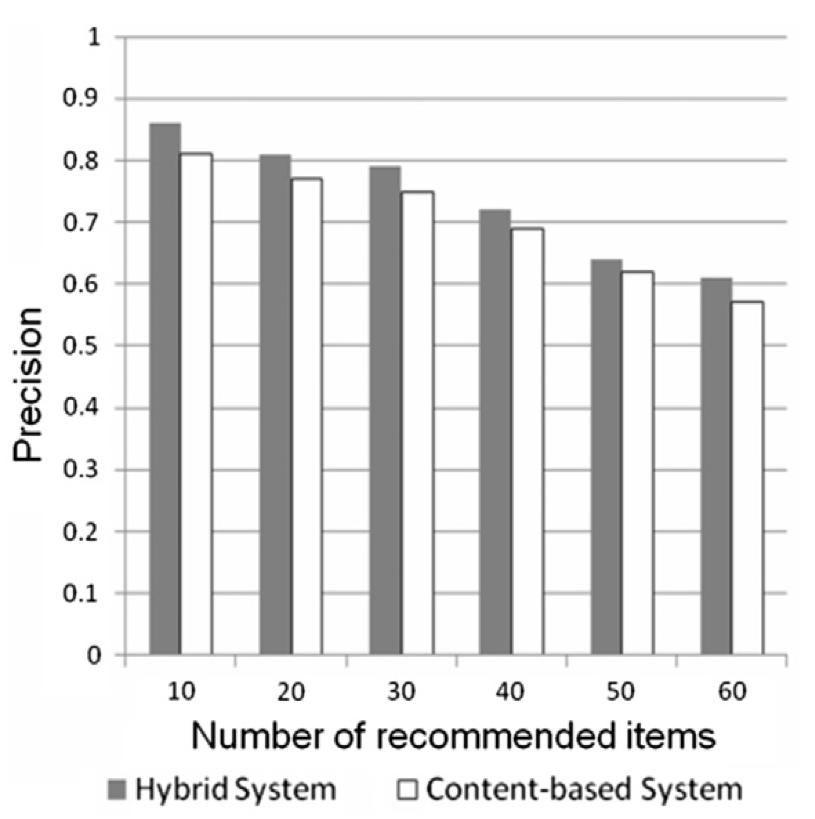
\includegraphics[width=80mm]{GFX/tech/hybridApproachPrecisionRate.png}
\caption{Precision rates showing the hybrid system versus the content-based system.}
\label{hybrid_approach_precision_rate}
\end{figure}

The user's interests are then matched with the contents of the news to present the recommended news item suited for the user. In figure \ref{hybrid_approach_precision_rate} the precision rates of the hybrid model versus the same system with just the collaborative filtering model approach is showing. The figure shows that the hybrid model has a higher precision than the collaborative filtering model.


\cite{liu2010personalized} also proposes a hybrid system where collaborative and content-based filtering are combined. A personalized news recommendation system for Google News is proposed. First a large-scale analysis of anonymized user click logs from Google News was conducted, to learn about the users' news interests. Further a Bayesian framework was developed to predict the users' current news interests based on activities of the current user and the trending topics based on the activity of all the users, found from the log analysis. At last, the content-based recommendation mechanism combined with an existing collaborative filtering mechanism is used to generate personalized news recommendations.

The presented hybrid system is then tested with Google News and shows that the quality of the recommendations are improved and the number of visitors have increased, compared to when just the existing collaborative filtering mechanism was used. 


\cite{das2007google} proposes a collaborative filtering approach for generating personalized recommendations for a large scaled system, namely Google News. These recommendations are generated following three approaches: Probabilistic Latent Semantic Indexing\cite{hofmann1999probabilistic}, MinHash\cite{broder1997resemblance} clustering, and co-visitation\footnote{Co-visitation means that two different articles have been visited by the same user in a defined period of time\cite{jannachrecommender}.} count.

\begin{figure}[!htbp]
\centering
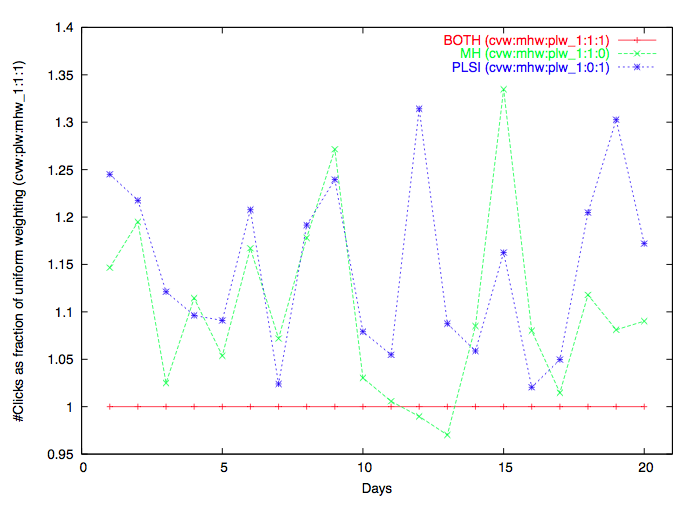
\includegraphics[width=100mm]{GFX/tech/googleNewsPersonalizationMinHashPLSI.png}
\caption{Live traffic click ratios for comparing PLSI and MinHash algorithms.}
\label{google_news_personalization_minhash_plsi}
\end{figure}

The test of the system used on a large fraction of the Google News traffic conducted over a period of several days, demonstrated the efficiency and scalability of the system, and figure \ref{google_news_personalization_minhash_plsi} shows that the algorithms MinHash and PLSI combined almost always performs worse than when run separately.


\subsection{Mobile News}

\cite{shapira2009epaper} describes a personalized mobile newspaper system called ePaper, a research prototype system which aggregates content from several different news providers. The news items are classified as concepts from a news domain ontology. Each subscribed user can then receive an electronic newspaper.

Ontological content-based and collaborative filtering algorithms are applied to the user's profiles and preferences to personalize the content from the newspapers. To maintain the user's profile, the user's activity log in the application are analyzed to provide an implicit and dynamic update. The user can also access a news paper reading experience without any form of personalization through ePaper.

\begin{figure}[!htbp]
\centering
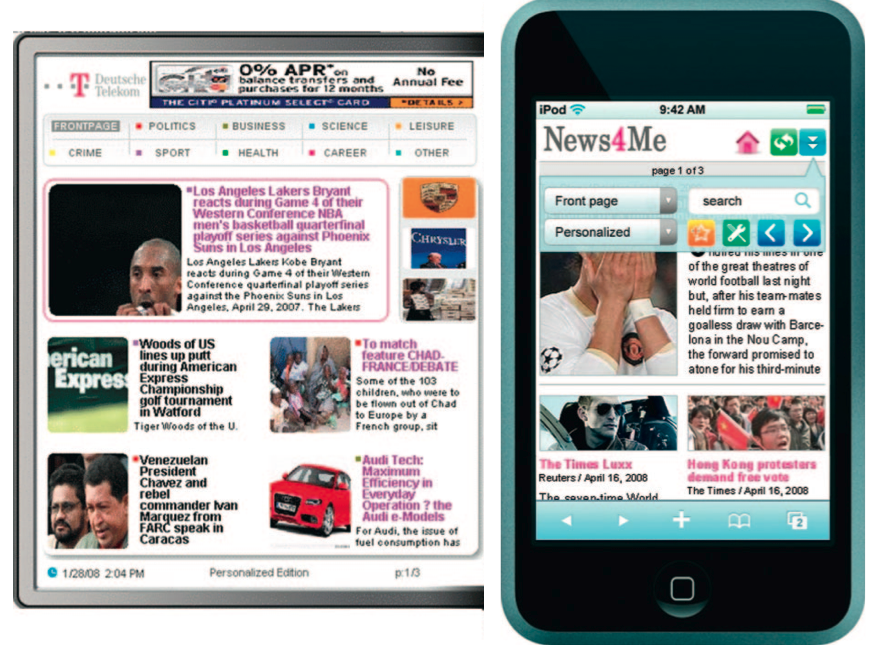
\includegraphics[width=100mm]{GFX/screenshots/ePaper.png}
\caption{The ePaper shown on two different devices.}
\label{screenshots_ePaper}
\end{figure}

The ePaper is designed in a responsive way, meaning that it is adapted to the screen size and specifications of the device it runs on, see figure \ref{screenshots_ePaper}.



\cite{lee2007moners} proposes a mobile web news recommendation system called MONERS. This system combines the nature of mobile web news content and service with the characteristics of users. 

A recommendation of a news article from MONERS is computed in several steps. The weight of an article is calculated by the degree of importance and the recency of that specific article. Users are assigned into category segments, where these segments are formed through k-mean clustering\cite{teknomo2006k} using Euclidian distance measure\cite{danielsson1980euclidean}. The change in the user interests, measured as the weights of a category preference at the user's side, determines which category segments this user belongs to. The article preference of a user segment is also computed. These computations forms the recommendation that is delivered to the user. Figure \ref{moners_flow_chart} shows the flow of the mobile recommendation system.

\begin{figure}[!htbp]
\centering
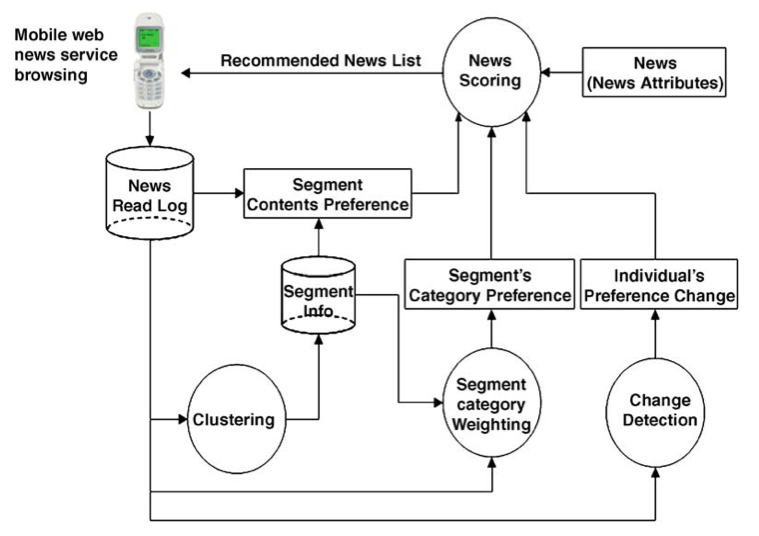
\includegraphics[width=100mm]{GFX/tech/monersFlowChart.png}
\caption{The flow chart of the MONERS mobile news recommendation system.}
\label{moners_flow_chart}
\end{figure}

MONERS was tested on real users of a mobile service operator and the result showed that the news accessed by category had more page hits, while the recommended news articles had a higher read ratio than articles sorted by recency or category.



\cite{yeung2010proactive} presents an Analytic Hierarchy Process\cite{saaty1988analytic} model as a fundamental part of a proactive personalized mobile news recommendation system. The AHP model's function is to rate the relevance of news items and it supports both collaborative filtering and content-based filtering. To estimate the user's level of interest, a Bayesian Network\cite{jensen1996introduction} approach is used. BN was chose because of its good performance, such as low memory usage and fast computations, as well as it helps solving the data sparsity problem. Further to push the proactive information, a hybrid P2P\cite{shen2010handbook} system is applied.

The proposed model is implemented as a mobile application in Java, named PPNews, supplying a just-in-time personalized news service. First the Bayesian Network is constructed, followed by the assignment of the weights and then the rank of each item is computed by applying the Analytic Hierarchy Process model.

The application was tested on 10 research staff members and students, resulting in positive feedback, such as battery life lasting almost a whole day using the application, as well as the news pushed was generally matching the user's profile.

\section{News consumption}
\cite{mashable2010newsconsumption} talks about how news consumption are shifting from accessing news from regular news sources on the Internet towards being presented and accessing news articles in a personalized manner via social news streams. A study done by Pew Internet on a sample of 2259 American adults, shows that approximately three fourths of the people asked who access news online, are accessing the news via email or posts on social networking sites\cite{purcell2010understanding}.

National Public Radio\footnote{National Public Radio is a public radio network serving over 900 public radio stations throughout the US.} also conducted a survey regarding social news consumption\cite{npr2010facebooksurvery}. NPR asked their Facebook fans, which then summed up to about one million people, if people use social networks to access news and information. With over 40 000 answers to the survey, 74.6 per cent agreed that "Facebook is a major way for me to receive news and information from NPR".

Although NPR's survey cannot say if the people who answered they survey is a good representative of the general public, it shows the same trend as the survey conducted by Pew Internet.

\section{Designing news applications}

\cite{vinod2010news} presents a news service called News Sync. The system was created focusing on three different scenarios of use, either separately or combined, namely news covering a topic, a location or within a specified time period. News Sync proposes a combination of NLP, machine learning, visualization and search to create a more "captivating and sticky news consumption experience".

\begin{figure}[!htbp]
\centering
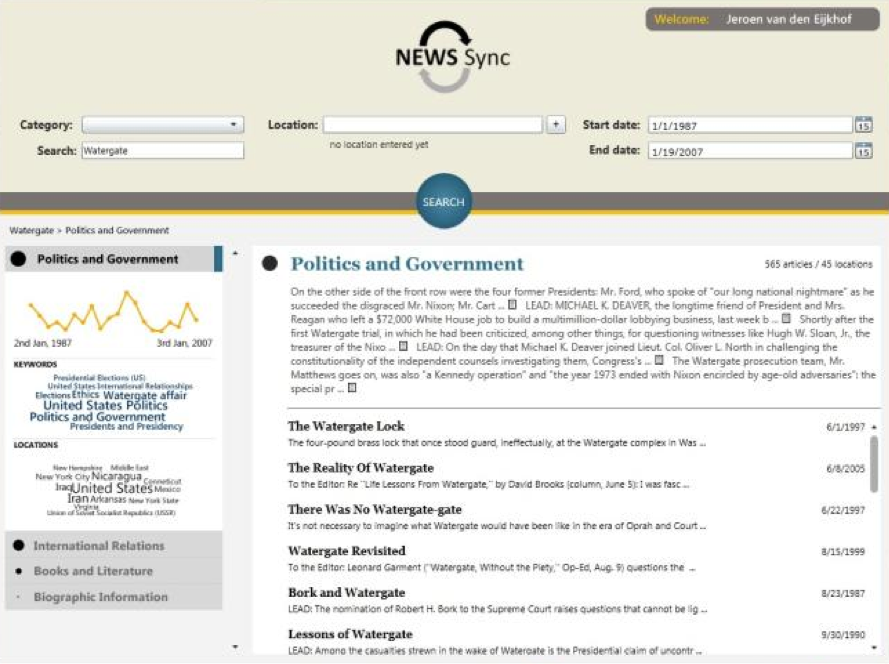
\includegraphics[width=140mm]{GFX/screenshots/newsSyncSearchWatergate.png}
\caption{Screenshot from News Sync showing the search result for Watergate.}
\label{news_sync_schematic_diagram}
\end{figure}

Figure \ref{news_sync_schematic_diagram} shows a screenshot of News Sync after a search for Watergate has been executed. The left-hand side consists of three main areas. A graph showing the distribution of articles containing the search phrase over the time specified, a tag cloud showing the keywords in the articles resulting from this search, and a tag cloud showing the locations concerning these articles. The higher concentration the bolder font, and all words in the tag clouds are clickable, for further browsing within this category or location.

The main view is showing the clustering of news articles from the selected keyword. The user can choose another keyword on the left-hand side, and another cluster of news articles will be shown in the main view containing articles within this cluster.

The user can share articles, summaries or stories to the most popular social networking sites, as well as saving the query for later access. All user activity are tracked and taken into account when building the personal profile, where this profile determines how the ranking and summarization of clusters are maintained to fit the user's profile.


\cite{anna2011designing} presents a proposal on how to design an aggregating news application, called 247, on the Apple's iPad device with focus on combining the credibility of the editor, a social media layer and a fluent interaction experience. A main concern is how to move the conventional newspaper onto a digital medium, and how the digital medium can be used in everyday life to access news, either as an individual catching up on the latest news, or as a peripheral device presenting the latest headlines to whoever is looking at the device.

It includes field work on how people are using the iPad as a device, and how, when and where people are accessing news throughout the day, resulting in a design allowing both individual use, and peripheral use (see figure \ref{future_of_news_individual_use} and \ref{future_of_news_peripheral_use}).

\begin{figure}[!htbp]
\centering
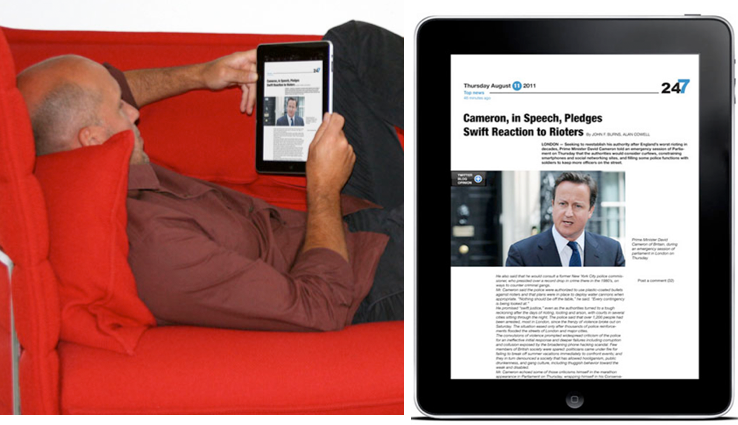
\includegraphics[width=120mm]{GFX/screenshots/futureOfNewsPaperIndividualUse.png}
\caption{Screenshot from 247 showing the individual UI design along with an example of individual usage.}
\label{future_of_news_individual_use}
\end{figure}

\begin{figure}[!htbp]
\centering
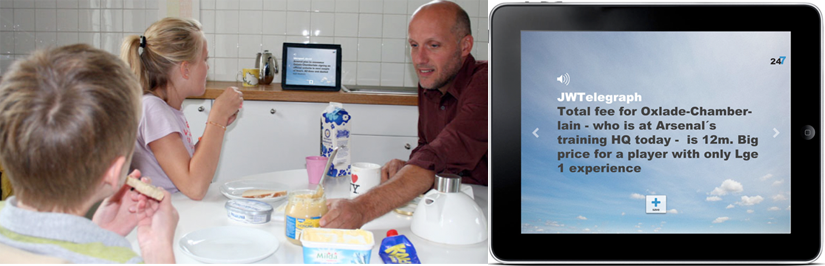
\includegraphics[width=120mm]{GFX/screenshots/futureOfNewsPaperPeripheralUse.png}
\caption{Screenshot from 247 showing the peripheral UI design along with an example of peripheral usage.}
\label{future_of_news_peripheral_use}
\end{figure}

\section{Commercial news recommender apps}
\label{commercial_news_applications}
There are a lot of different commercial news recommender apps, and since these are commercial systems, only a limited amount of information about their underlying technology has been published.

Following are a short description of ten of the most popular and well known mobile news applications that are available at this time of writing, subjecting both the UI and how the recommendation is solved, if obtainable.

\subsection{Zite}
Zite is an intelligent magazine, which aims to guide the user towards discovering interesting things to read\cite{zite_appstore}.

\subsubsection{User Interface Design}
The Zite application meets the user with an infinite vertical scrollable view consisting of the top stories. Each news story is framed within a rectangular tile, whereas each tile consists of at least a title and the publisher of the article. The tile can also include tags, lead text, the time since it was published and the article's image (see the first image in figure \ref{screenshots_zite}).

From the top stories the user has several choices. In the top left corner the user can access his "quicklist" of categories and entities (see the last picture in figure \ref{screenshots_zite}). In the top right corner the user can search for topics like music or entities like Rolling Stones. These search results can be added to the "quicklist" to access them later. If an article is tapped, that article is showed in a new view (middle picture in figure \ref{screenshots_zite}). Here the user can read the Zite's version of the article or open the publisher's version. The user can share the article through numerous social websites and services. The article can be rated with thumbs up or thumbs down buttons. The user also has the ability to change the text size of the article or block the publisher of the article to never get another article from this publisher from this screen.

Zite has a clean and simple UI design with a minimum of surprises regarding navigation. All is more or less straight forward, with an exception of the swipe left on the main screen to trigger the next element on the "quicklist", which might come as a surprise to the common user.

\begin{figure}[!htbp]
\centering
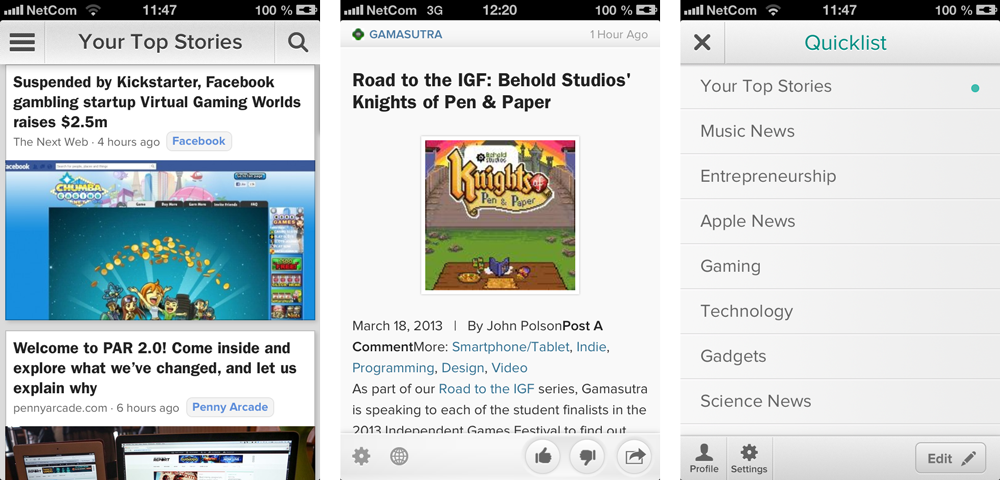
\includegraphics[width=130mm]{GFX/screenshots/zite.png}
\caption{Screenshots from Zite showing the Top Stories feed, a single news article, and categories list.}
\label{screenshots_zite}
\end{figure}

\subsubsection{Technology}
Zite uses different approaches to personalize the news magazine for the user\cite{zite_faq}. It uses automated algorithms to retrieve articles that are trending now by looking at how the different articles are discussed and shared on different websites, blogs, popular social network services, like Twitter and Facebook, and other news applications like Pocket and Google Reader. If an article is considered less trending by the algorithm, it is less likely to appear in the news stream, although the user might consider this article interesting.

The user can also choose to login with one or more of the aforementioned social network services and news applications, and get news recommendations based on what is shared by the user itself and friends of the user, or based on what is stored by the user in the news applications. 

Zite offers to save the user profile so the user can access its personalized news feed on different devices, but it does not limit the use of the application if a user chooses not to sign in.

The user can heavily influence what kind of news that are retrieved by rating different articles with the "thumbs up" or "thumbs down" buttons. The more rating the user gives, the better the personalization gets. Zite also keeps track of which articles the user is reading and which articles that are shared by the user and the user's connections on the social networks. This tracking influences the content delivered to the user.

In addition the user can search for different entities of interests, and further choose to like this type of entity by clicking a heart shaped button. If it is liked, this type of news will start to show in the main news stream. The user can also choose to add this entity to the "quicklist" to be able to quickly access only this type of news in the news stream.

A single source can also be blocked completely, as explained in the previous section.



\subsection{Flipboard}
Flipboard is a digital news magazine combining news of all sorts and events and feeds from social networks. Flipboard has gained much attention because of their joyful and easy-to-use flip-design.

\subsubsection{User Interface Design}
When launched, Flipboard greets the user with a front page consisting of different categories (see left image in figure \ref{screenshots_flipboard}). These categories are set by the user by clicking the "Your Flipboard" button shown in the right picture in figure \ref{screenshots_flipboard}. This settings screen is triggered by clicking the red ribbon in the top right corner of the start screen. While in the start screen the user can navigate further down by swiping or clicking one of the categories.

When a category is tapped, news articles from this category can be browsed by swiping up or down. Each category stream uses a full size view for each article, meaning that one article's preview uses the whole mobile screen. Each article's preview shows at least the title of the article, publisher and/or author, and the time since it was published. The preview can also include an image, lead text, and how many retweets\footnote{A retweet is if someone on Twitter shares a Twitter message created by someone else.} this article has. The user can also bring up the settings screen from this screen by tapping the magnifying glass in the top right corner.

When the article's preview is tapped, the user is presented with the article screen (see the middle picture in figure \ref{screenshots_flipboard}). Here the user can swipe up and down to read the whole story. If the article is retrieved from a social network, the user has the opportunity to interact with the social network the article is gathered from, like retweet and favorite for Twitter or "like" for Facebook. The user also has the ability to share the article via other services or choose to read it later by clicking the "out of the box" arrow on the top.

Flipboard has an easy to use interface design, and has gotten a lot of attention because the app is considered to have a beautiful design\cite{flipboard_design} and a special flip-like animation that is used when scrolling the pages.\cite{flipboard_video}\cite{flipboard_animation}. Flipboard was also picked as "App of the Year" by Apple in 2010\cite{flipboard_app_of_the_year}.

\begin{figure}[!htbp]
\centering
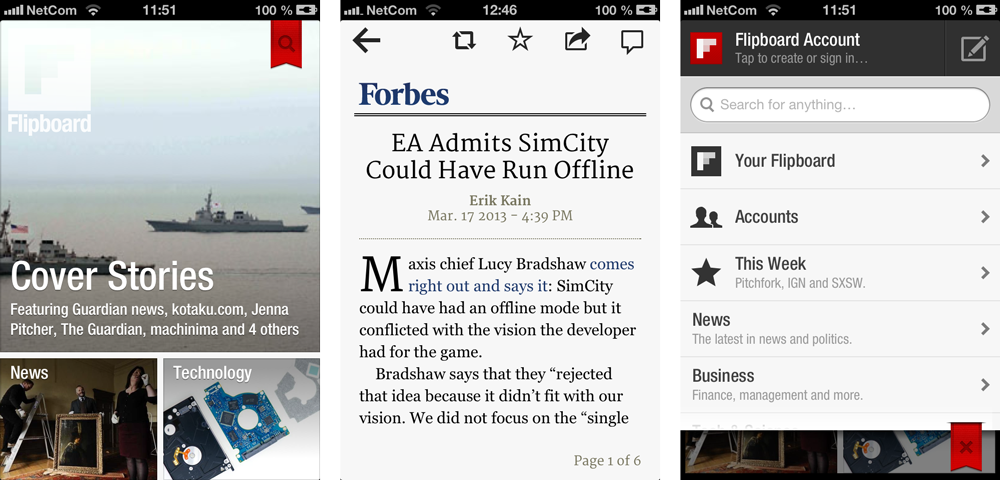
\includegraphics[width=130mm]{GFX/screenshots/flipboard.png}
\caption{Screenshots from Flipboard showing the top categories, a single news article, and the settings view.}
\label{screenshots_flipboard}
\end{figure}

\subsubsection{Technology}
Flipboard allows users to include their own social feeds from Twitter, Facebook, Google+, along with RSS feeds. Flipboard also crawls the Internet for trending news articles and categorizes them accordingly.

Flipboard acquired the Ellerdale startup early on\cite{flipboard_acquired_ellerdale}. The Ellerdale project included a semantic data-analysis technology which started as a Twitter trend analysis before it was acquired by Flipboard. Using Twitter's firehose API\footnote{The Twitter Firehose API allows third party developers to get access to all tweets that are composed in real-time.} the Ellerdale Project was able to process all tweets, thousands per second, and categorize them by topic, rather than keywords\cite{flipboard_categorize_by_topic} being able, in theory, to differentiate between Internet Explorer, Ford Explorer and Dora the Explorer. Further on Flipboard uses this technology to crawl social networks for trending topics and news, and being able to categorize them by topics to present useful and interesting news to the user.

The application offers the user the ability to create a Flipboard account to be able to access the personal feed on several devices. The application is still highly usable without creating an account, but some of the functionality is limited when not logged in. For instance, the user cannot save articles for later reading, like or comment articles without signing in.

\subsection{Pulse}

Pulse is a news reading application for iOS, Android and web browsers that supports HTML 5. It was released for the first time in 2010 and was awarded with the Apple Design Award of 2011\cite{pulse_apple_design_award}.

\subsubsection{User Interface Design}

When first booted, a login is required, either by a Pulse account or via Facebook. When logged in the first time, the user is presented with a limited set of news categories which the user can choose from to add to its interests. 

When done selecting category interests, the user is met with the main view, which is shown as the start up screen from now on, as shown in the first image in figure \ref{screenshots_pulse}. This screen shows one category with several publishers sorted in rows. By swiping horizontally in a publishers row, the user can browse the different articles from this publisher. By swiping vertically the user can browse the different publishers in this category. If the user swipes to the bottom of the screen, it can click the "Add Content" button, and add more sources of liking.

The sources can be removed by tapping the "Edit" button in the top right corner, and to change the displaying category, the user can hit the menu button in the top left corner. The user then has the ability to select another category (see the last image in figure \ref{screenshots_pulse}), or add more content to the news feeds.

The main screen has a lot of information showing at the same time and can feel somewhat cluttered and overloaded.

When an article is tapped, the single article screen is presented (see the middle image in figure \ref{screenshots_pulse}) to the user. This screen shows whatever information available from the source feed, like title, author, when the article was published, image and a lead text or article text if available. By hitting the action button in the top right corner, the user has the ability to save the article for later reading or sharing via Facebook, Twitter or email. 

By swiping horizontally the user can switch between the different articles from the showing publisher, similarly to the main screen. The user also has the ability to show the whole article by either tapping the title or pressing the "Read on Web" button at the bottom of the article. By doing so, the full article is presented in a web view, showing the publishers own website with the given article.

\begin{figure}[!htbp]
\centering
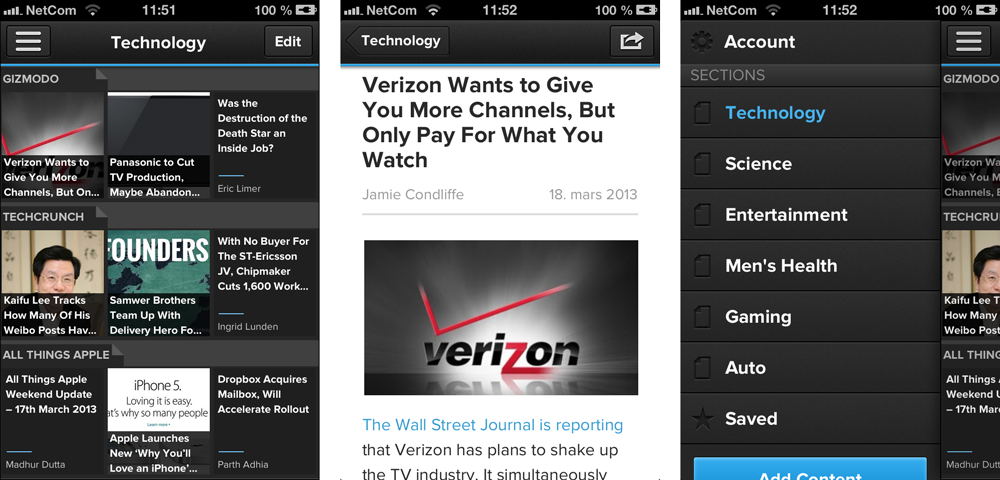
\includegraphics[width=130mm]{GFX/screenshots/pulse.png}
\caption{Screenshots from Pulse showing the start page, a single news article, and the categories/settings view.}
\label{screenshots_pulse}
\end{figure}

\subsubsection{Technology}

On first startup, after login, Pulse lets the user choose from a dozen or so different categories to start off the news reading experience. These different categories gets news from different predefined sources added by the developers. 

Pulse is mainly based on news publisher's RSS feeds, but allows the user to add their own social feeds from several social networking sites, e.g. Instagram, Facebook and YouTube.

The application also has the ability to search for feeds and add personal RSS feeds to a predefined category or a custom category. This way a user can add the newspaper feeds of their interests. Pulse can also check for the devices location and search for feeds that are nearby by using the GPS coordinates.

If logged in with Facebook, Pulse crawls the users news feed and finds articles previously shared or otherwise interacted with, and shows these article's sources in the recommended section.


\subsection{Summly}

Summly is a gesture oriented news aggregating application which was developed by Nick D'Aloisio in 2011. The main idea was not to personalize the news reading experience, but rather create intelligent summaries of the most trending news, by using advanced text analysis and natural language processing methods\cite{summly_idea}. Summly was sold to Yahoo! for reported £18 million GBP in March 2013\cite{summly_sold_yahoo}, and was shortly after removed from the App Store, for Yahoo! to use the summary technology elsewhere\cite{summly_closed}. On April 22nd, Yahoo! released their new news application using the NLP algorithms and machine learning that previously was used in Summly\cite{yahoo_news_app_release}

\subsubsection{User Interface Design}

The front page in the Summly application shows the user how many unread Summlys\footnote{A Summly is a summarized version of a website or article.} (s)he has. It also shows the title, publisher and category of a trending article as of now. The title of the trending article is also a button, and when clicked, the application opens the single article view showing the clicked article. 

The single article view (see the second image in figure \ref{screenshots_summly}) shows the article's image, title, publisher, time since it was published, number of words in the full Summly and the short Summly. With horizontal swipes the user can navigate between different articles in the current showing category. To read the full Summly the user can double tap the anywhere on the screen. In the full summary the user can choose to close the full Summly by double tapping the screen again or open the article at the publisher's website in a web view by tapping a blue right arrow button.

In the single article view the user can also access the full article at the publisher's site by swiping down. To share or save this article, the user simply holds down one finger and a share view is presented where the user can save the article, or share it on Twitter, Facebook or mail.

By swiping up in the single article view the category view (first image in figure \ref{screenshots_summly}) is shown. Here the user can choose to read from another category or add new categories, entities or topics by clicking the plus button at the bottom of the category screen. The screen where categories are managed are shown in the last image in figure \ref{screenshots_summly}.

\begin{figure}[!htbp]
\centering
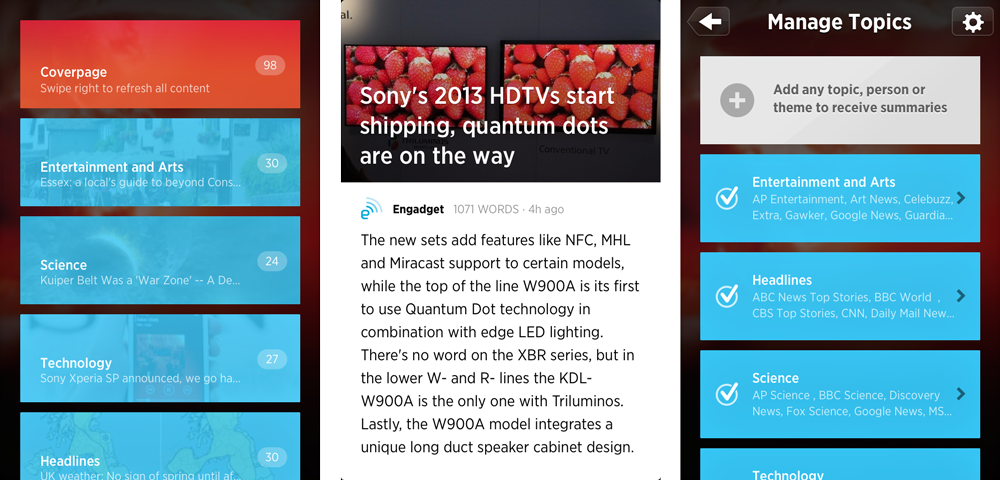
\includegraphics[width=130mm]{GFX/screenshots/summly.png}
\caption{Screenshots from Summly showing the category selection page, a single news article, and the category settings view.}
\label{screenshots_summly}
\end{figure}

\subsubsection{Technology}

Summly has the ability to add custom categories, topics and entities as well as giving the user the latest and most trending news within these categories, topics and entities. Summly does not focus on personalization or recommendation, but rather on creating intelligent summaries of news articles, as earlier mentioned. 

Summly states when talking about how the text summarization is done: "instead of a robotic, linear algorithm, Summly uses a genetic algorithm to mimic how a human actually thinks, using organic metrics to extract the most critical components"\cite{summly_launch_video}. Summly uses an advanced algorithm based on machine learning and NLP to create their 400 character long summaries of the news articles. At first the summarization technique was rather basic, but it got more complex when Summly teamed up with SRI International\cite{summly_technology}.

As a result to not focusing on personalization and news recommendation, Summly does not have any form for log in other than using the built in sharing capabilities for Twitter and Facebook that already is present in iOS.

\subsection{News360}

News360 is a news recommendation application and according to themselves a "smart and elegant app that learns what you like and brings you stories from across the web"\cite{news360_about}, available for iOS, Android and the Windows 8 series.

\subsubsection{User Interface Design}
On the first load, the user can choose to log in or continue without an account. Next, the user is prompted with a set of categories to select as interesting, a possibility to search for other entities to add to the feed, and an option to crawl the user's social news feeds for articles interacted with to add these topics to the personalization feed.

When the personal news feed is finished building, the home screen is presented to the user (see the first image in figure \ref{screenshots_news360}). This is also the first screen that meets the user when the application is launched after the initial setup is done the first time. News360 shows one news article per screen, and horizontal swiping is used to navigate to other stories. This screen shows the article image, if any, which category the story resides to, the title, publisher, how long ago since it was published and how many similar or related stories News360 has indexed.

By swiping down on this screen, the user can access the share screen, the "thumbs up" and "thumbs down" buttons to rate the article, and a save button, if the user wants to read the article later. By swiping up the user is presented with the lead text of the article and from here can choose to read the whole article by tapping the article or by hitting the "Continue" button.

When the single news article view is presented, the user has the same action buttons as by swiping down on the previous view, share, rate and save (see the second image in figure \ref{screenshots_news360} in the top right section.). In this view the user can choose to read more of the story, view the story from the publishers website, or choose a similar story by another publisher, to get the story from another angle or view. The user can also get more stories from this publisher by clicking the publisher's name. If the publishers name is tapped, the user can navigate to other stories by this publisher, see the publishers profile and choose to subscribe to this publisher.

By tapping the button in the top left corner in the main view (see first image in figure \ref{screenshots_news360}), the menu view is shown (see the last picture in figure \ref{screenshots_news360}). From here the user can navigate to the other categories or entities that it has added. The user can also get news by location, edit existing topics, add new topics, search for news, read saved stories, log in or out, and navigate to the settings section.


\begin{figure}[!htbp]
\centering
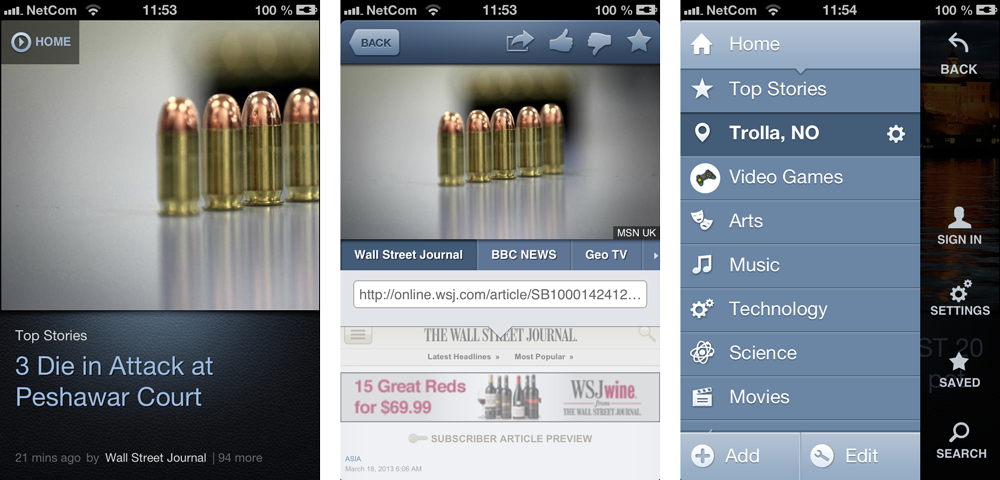
\includegraphics[width=130mm]{GFX/screenshots/news360.png}
\caption{Screenshots from News360 showing the top stories feed, a single news article, and the category settings/selection view.}
\label{screenshots_news360}
\end{figure}

\subsubsection{Technology}
News360 uses a lot of advanced technology to be able to recommend news to the reader\cite{news360_technology}. The semantic analysis platform is created from seven years of natural language analysis and development experience. News360 uses a self made sophisticated linguistic analysis engine to perform tasks like entity extraction, fact extraction, text classification, dossier generation and clustering.

Further this engine is used in combination with a complex news-gathering system to analyze more than 100 000 articles a day in real time. From this analysis approximately 700 000 different people, locations, brands and companies are identified. Then the articles are tagged with locality and topics, and stored in clusters.

To understand which stories that are important, News360 uses a ranking algorithm which checks the impact of the sources that are aggregated, and all the articles that are published in that source. The system also checks the audience and credibility of the source and author, text characteristics and the velocity of the news event as it is happening.

News360 also gives the user the ability to tailor these recommended news by letting the application check the user's social feeds to find articles and sources interacted with. The user can rate each article with "thumbs up" or "thumbs down" buttons to have an impact on which news are shown.

With their semantic analysis, News360 also offers the user the ability to read similar stories, but from different publishers, to have the ability to view the news event from several points of view and angles.

A summary of the work flow, gathered from \cite{news360_technology}, is shown in figure \ref{tech_news360_workflow}.



\begin{figure}[!htbp]
\centering
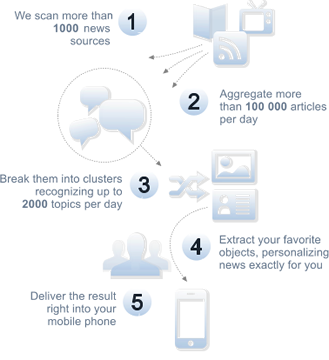
\includegraphics[width=70mm]{GFX/tech/news360workflow.png}
\caption{The workflow of the News360 news system}
\label{tech_news360_workflow}
\end{figure}


\subsection{Circa}
Circa is a mobile news application for the iPhone that summarizes news for the user by using real editors on the most trending news and breaking these news stories down to short paragraphs and bullet points\cite{circa_about}.

\subsubsection{User Interface Design}
When first loaded, the user can login, create an account, login with Facebook or choose not to log in at all.

Circa has three main views, the news feed, the single news view, and the category selection view, which is shown in the three images in figure \ref{screenshots_circa} respectively.

The news feed is the start screen when the application is launched. The user is presented with images from the most recent and trending news at the top in a horizontal scrollable view, followed by an endless vertical scrollable view with news stories from the category chosen. From here the user can browse through more news stories by swiping up in the vertical scrollable view.

To enter the whole story (second picture in figure \ref{screenshots_circa}) the news story has to be tapped. The single news view has three buttons in the top right corner. The first, an "i" button, shows which sources Circa's editors has used to create the summaries that are presented to the user. These sources are also clickable, if the user wants to open the whole article in a web view. The second, a share button, lets the user share the whole article or some part of the summary via Facebook, Twitter, mail or SMS. The last, a plus button, lets a user subscribe to the news story, meaning that the user will be notified if there is new information added to the news story, which happens when an editor changes a news article in some way.

To head back to the news feed the user can either tap the back arrow in the top left corner, or swipe right. To bring up the category view (last image in figure \ref{screenshots_circa}, a user simply taps the button in the top left corner in the news feed view or swipes to the right. Here the user can choose another category by tapping the wanted one and the chosen category will be loaded and shown in the news feed.

\begin{figure}[!htbp]
\centering
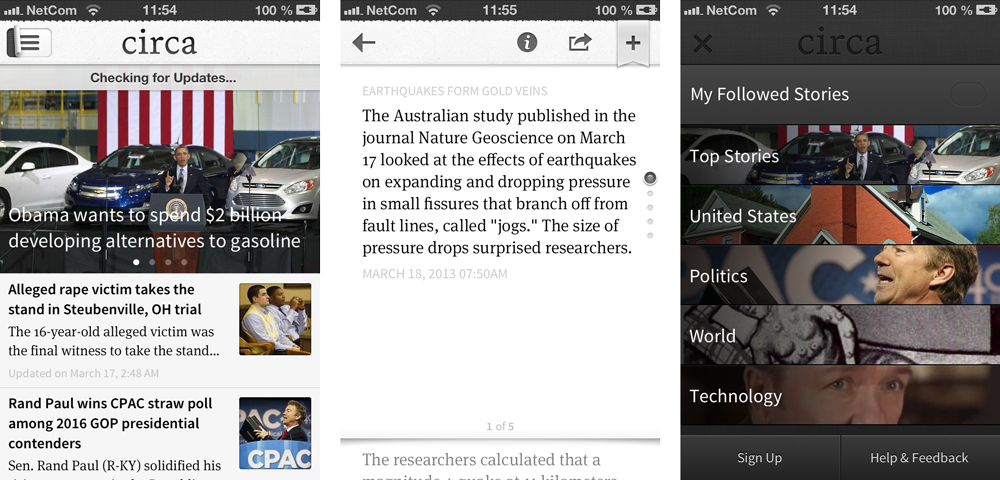
\includegraphics[width=130mm]{GFX/screenshots/circa.png}
\caption{Screenshots from Circa showing the top stories feed, a single news article, and the category selection view.}
\label{screenshots_circa}
\end{figure}

\subsubsection{Technology}
Similar to Summly, Circa does not focus on the personalization and recommendation part of the news reading experience, but more on the part of bringing the most essential parts of a news article to the user by creating summaries.

While Summly uses NLP and machine learning to do so, Circa has an own editorial staff, working solely with creating summaries for the news reader, in terms of bullet points, facts, quotes, photos, maps and related stories\cite{circa_about}.

\subsection{Wavii}
Wavii is something in between a news application and a social network application, and has been called "A Facebook for Topics"\cite{wavii_facebook_for_topics}. The main idea is that a user can follow topics and interact with these topics, rather than friends on Facebook, for instance. The user gets a news feed of interesting topics, where the sources of these news feed instances can be news sites, Twitter, blogs, etc., and the user can share his/hers reaction to the story, comment and share with friends. In April 2013, Wavii was acquired by Google, and later removed from the app market for their NLP technology to be used in Google's own products\cite{google_acquired_wavii}.

\subsubsection{User Interface Design}
To be able to start using Wavii, the user has to login, either using Twitter, Facebook or by creating a Wavii account with an email address. After login the user is prompted with a screen to start following topics.

The start screen is a news feed showing followed topics and is an aggregated endless feed of all topics that is followed (see first image in figure \ref{screenshots_wavii}). Each story in the feed is an event and includes one or more topics that is followed. The story can be interacted with in several different ways, like share reaction in terms of different predefined facial expressions shown as simple drawings, commenting, sharing on social networks and poll questions.

The top bar is scrollable in a horizontal direction, and here the user can change the main category of the news feed, in terms of categories extracted from the different topics followed. By hitting the menu button in the top left corner, the navigation view, shown in last image in figure \ref{screenshots_wavii}, is revealed. Here the user can navigate to the different main views of the application, like the main feed, user profile, discover new topics, search for friends and settings.

When a story in the main feed is tapped, the single story view, shown in the second image in figure \ref{screenshots_wavii}, is shown. In the single story view the news story, twitter feed, or whatever the source of this event is, is shown. The user also has the ability to read a part of the source that caused the event, or open the whole source in a web view. The single story view also shows which stories or events that are concerning the showing event, in terms of clickable boxes, and lets the user follow that story or event by simply clicking it. At the bottom of the single story view, a dozen of related topics and events are shown, these also as boxes, and by clicking these the user can easily start following it.

\begin{figure}[!htbp]
\centering
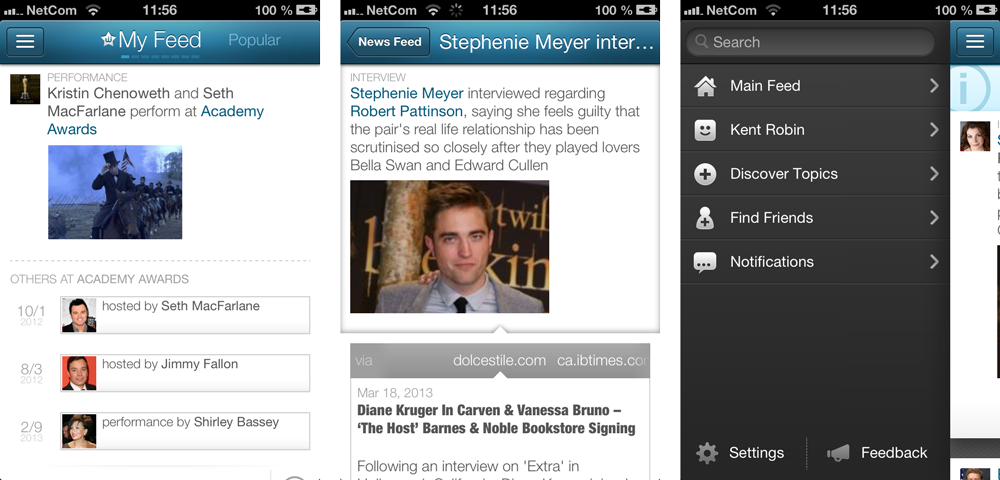
\includegraphics[width=130mm]{GFX/screenshots/wavii.png}
\caption{Screenshots from Wavii showing the top stories feed, a single news article, and the category selection/settings view.}
\label{screenshots_wavii}
\end{figure}

\subsubsection{Technology}
To help you find interesting topics, Wavii can crawl the user's social feeds, and propose a set of topics to follow, based on what the user and the friends of the user has interacted with. The user can also search for topics to follow.

To extract topics and events, Wavii uses a proprietary algorithm for NLP\cite{wavii_proprietary_algorithm}. Oren Etzioni, a professor in computer science and a specialist in the field of AI, at the University of Washington, who also is an advisor to Wavii, says that Wavii uses a state-of-the-art extraction algorithm to gather topics and events\cite{wavii_facebook_for_topics}.

\subsection{Prismatic}
Prismatic is a news recommendation application that gives the user a personalized news feed based on social network aggregation and applies machine learning algorithms to filter content based on the user's interests\cite{prismatic_wikipedia}.

\subsubsection{User Interface Design}
To get started with Prismatic, the user has to login, either with Facebook, Google+ or Twitter. The user can also register a "Stealth"-account, as Prismatic calls it, if the user do not want to connect the application with their social account.

When logged in for the first time the user starts a tour of the application to add interests and get to know how to use the application. The interests suggestions are based on localization and the user's social network feeds and interactions. The user can also search for topics to be included in the news feed.

The news feed is shown in the first image in figure \ref{screenshots_prismatic}, and this is also the main screen of the application. Here the user is greeted with an endless feed of news stories based on the user's interests. Each story can have a title, an image, the source of the story, a lead text and zero or more topics or entities that is connected to the story.

When a story is tapped the story is presented in the single news view, as shown in the second image in figure \ref{screenshots_prismatic}. Here the user can read the whole story in a vertical scroll view, get a list of related stories by tapping the text that states how many related stories there are and open the sources for the story in a web view by tapping the keyword associated with this source. 

A press and hold gesture wherever in the application will bring up three action buttons to interact with the selected news story. The three buttons are save the story for later reading, add the story to the favorites list, and share the story. If the share button is clicked, it will bring up a new screen, where the user can share the story by email, Facebook or Twitter.

By swiping left anywhere in the application, the category selection/settings view is brought up, shown in the last image in figure \ref{screenshots_prismatic}. Here the user can search for new topics or sources, deselect already chosen topics or sources, access the user's activity in terms of articles that are shared, saved, read and starred, and get suggestions for new stories, topics and sources. 

\begin{figure}[!htbp]
\centering
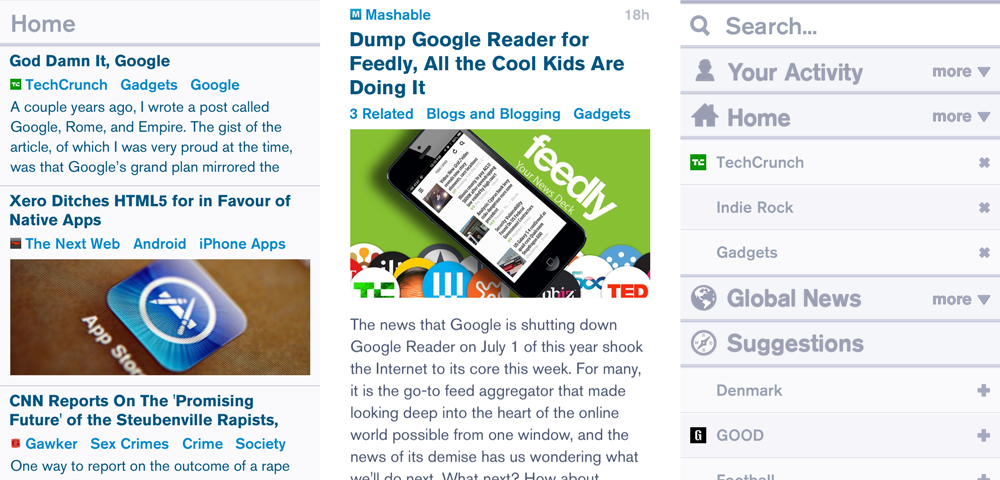
\includegraphics[width=130mm]{GFX/screenshots/prismatic.png}
\caption{Screenshots from Prismatic showing the top stories feed, a single news article, and the category selection/settings view.}
\label{screenshots_prismatic}
\end{figure}

\subsubsection{Technology}
Instead of just crawling the user's social feeds for news that are shared or otherwise interacted with by the user or the user's friends, Prismatic categorizes and extracts keywords and entities from those news and finds news that are related to the news that are shared. Prismatic also tracks all the moves the users does to further build the user's interest profile. Each user profile has a set of stored interests with a weight of how important that interest is, illustrated in figure \ref{prismatic_interest_bubbles}. The user profiles are also updated in real time, and the news reading habits of the user will immediately affect the user's profile and which news that are recommended\cite{prismatic_how_it_works}.

\begin{figure}[!htbp]
\centering
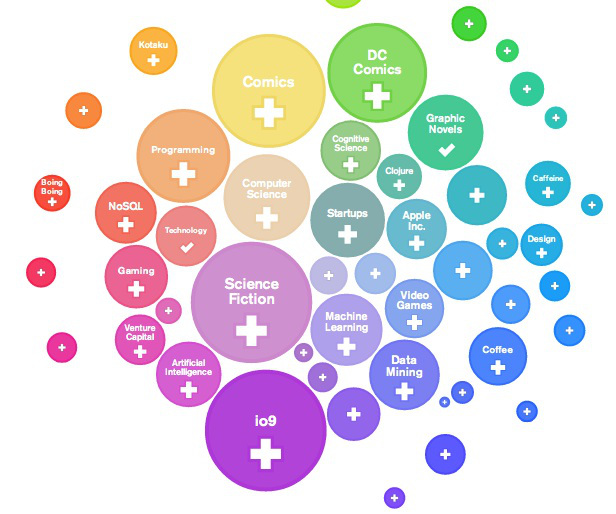
\includegraphics[width=130mm]{GFX/tech/prismaticInterestsBubbles.jpg}
\caption{An illustration of how the prismatic user's interest profile are stored created by Aria Haghighi, co-founder of Prismatic.}
\label{prismatic_interest_bubbles}
\end{figure}

To gather source for the news articles, Prismatic fetches millions of new news articles, blog posts, as well as other type of shared content, every day. All these sources are analyzed and processed with the use of machine learning and machine language training\cite{prismatic_how_it_works}.

\subsection{Taptu}
Taptu is a social news aggregating application with the slogan "DJ your News". This means that the user can create their own stream, combine or split streams or add your social network feeds as own streams inside the application. The application comes with a lot of predefined feeds from a lot of different sources, sorted by categories, but the user can also search for other streams as well. Taptu is available for iOS, Android and web.

\subsubsection{User Interface Design}
At the initial launch, Taptu offers to connect the application with Facebook, Twitter, LinkedIn or Twitter. Further the user can choose topics of interests to be included in the news feed. This also includes the user's social news feed, if the user chose to connect with one or more of the social networks.

The main view which holds all the different feeds are shown in the first image in figure \ref{screenshots_taptu}. Each feed is horizontal scrollable to browse the different news stories in this feed. All the feeds are put in a vertical scrollable view to be able to access all the different feeds. At the bottom there are four buttons, namely "Streams", "StreamStudio", "Add Streams" and "Settings".

The "Streams"-button shows the main view, just described. The "StreamStudio"-button shows a view where the user can manage the streams, like merge, split, rename, and remove sources from the stream. When the "Add Streams"-button is tapped, the view shown in the last image in figure \ref{screenshots_taptu} is presented. Here the user can add streams from one of the predefined categories by tapping the desired stream. The user can also search for other streams, or choose to login with Google Reader to include streams the user already has created in Google Reader. The last button shows the settings view where the user can change the layout of the application to his/her liking, in terms of fonts, text size, and background color. The user can also manage the social user profiles and feeds in this section.

In the second image in figure \ref{screenshots_taptu}, the single article view is shown in a vertical scroll view. This view can consist of an image, title, author, and a text. At the bottom of the scroll view, Taptu also lists a couple of related topics which the user can chose to follow by tapping them. At the bottom of the page there are three buttons, the "Globe"-, "Star"-, and "Arrow"-buttons. The "Globe"-button opens the showing article in web view and shows the original article at the news provider's web page. The "Star"-button adds the article to a bookmarks stream for easy access later. The "Arrow"-button or "Action"-button, as it is often called, brings up a share screen where the user can share the story via numerous different channels, like email, Twitter, Facebook, and LinkedIn.

\begin{figure}[!htbp]
\centering
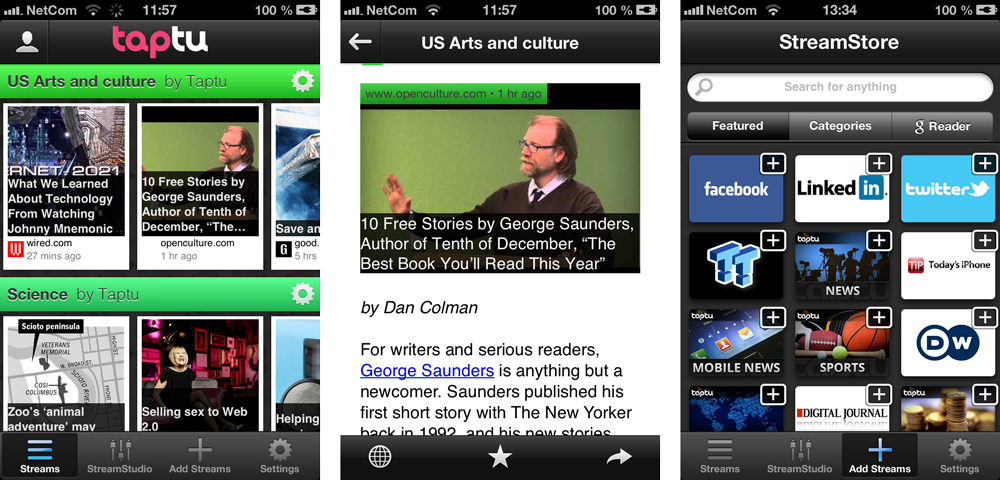
\includegraphics[width=130mm]{GFX/screenshots/taptu.png}
\caption{Screenshots from Taptu showing the top stories feed, a single news article, and the category settings view.}
\label{screenshots_taptu}
\end{figure}

\subsubsection{Technology}
Taptu crawls social networks and retrieves the most shared news and posts, and lets users add own streams, in addition to the predefined streams, but Taptu does not have any advanced form of personalized recommendation. Their approach is more towards letting the users themselves choose what kind of sources to be displayed.

It does however lets the user enable an option to the streams that is called "Taptu Magic", which follows the user's reading habits and shift articles more and more towards a subject that is more read than another\cite{taptu_magic}. For instance, if a user has a sports stream, and the user reads in general more basketball news than baseball news, "Taptu Magic" will start showing more basketball news and less baseball news in this stream.

\subsection{Feedly}
Feedly is a news aggregator application for iOS, Android and web. It is quite similar to Taptu in terms of functionality and purpose. Basically it is an advanced RSS-reading application.

\subsubsection{User Interface Design}
On the initial load, Feedly gives the user a quick introduction to the application and points the user in the direction of how to add feeds to the application. The application is highly usable without any login, but if the user wants to add own feeds and store these to later, a sign up with Google is required.

To find new feeds, the user can search by keywords in the search field or by browsing the predefined topics, as shown in the last image in figure \ref{screenshots_feedly}. If the user has signed in, a source can be added to a feed, otherwise the previous feed that was shown will be replaced by the new feed that is selected.

The main screen, shown in the first image in figure \ref{screenshots_feedly}, consists of a news feed contained in a vertical scroll view and a toolbar at the top. The toolbar has four buttons, the menu, title, add, and search button. 

The menu button in the top left corner, shows a category selection and settings menu if the user is signed in. If not, the user is prompted to sign in via Google. When signed in the user can navigate to the different feeds, show all feeds as an aggregated feed, manage feeds, add new content, and change Feedly application settings.

The title, in the top middle, also works as a button. When tapped it brings the user to the start of the feed again.

The add button, lets the user add the current displaying feed to an already defined category or to a new one.

The search button is located in the top right corner, and this opens the search view shown in the third image in figure \ref{screenshots_feedly}.

When a single article is tapped in the main view, the single article view, as shown in the second image in figure \ref{screenshots_feedly}, is brought up. The single article view has a toolbar at the top with four buttons, and a vertical scroll view which shows whatever information is available from that feed, like title, number of likes, author, time since it was published, image, video, lead text, full article text. At the bottom of the scroll view there is a button to open the article at the publishers site in a web view.

The four buttons at the top consists of a back button, which takes the user to the previous page, a custom button which is set by the user, a save button and a share button.
The custom button can be, for instance, share to Twitter or open in Safari. The save button stores the article for accessing later or via another device. The share button opens a small view with numerous different buttons to share via different services, like Facebook, Google+, buffer, mail, and Instapaper.

\begin{figure}[!htbp]
\centering
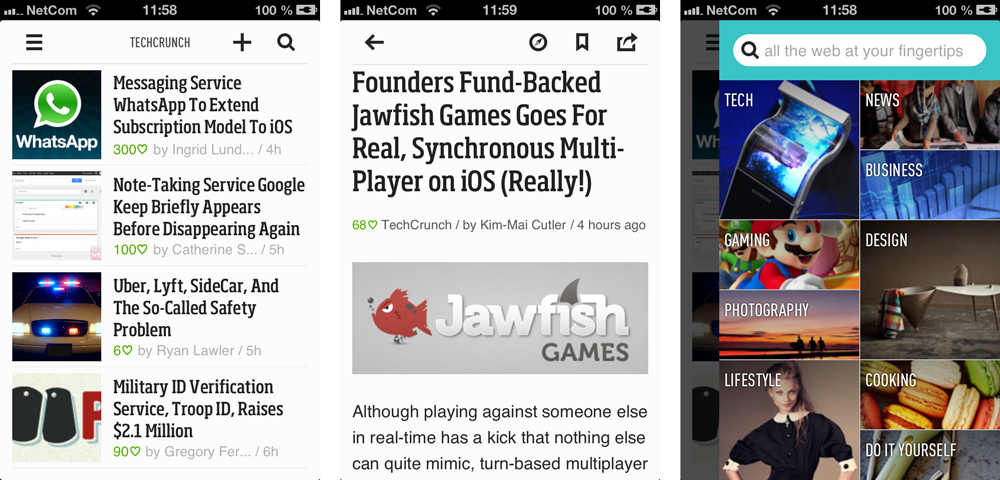
\includegraphics[width=130mm]{GFX/screenshots/feedly.png}
\caption{Screenshots from Feedly showing the top stories feed, a single news article, and the category settings view.}
\label{screenshots_feedly}
\end{figure}

\subsubsection{Technology}
As Feedly is more of an advanced RSS-reader, than a news recommendation application, and the focus of the application seems to be on creating a highly functional one, Feedly lets the user be in total control of the content, and does not offer any personalized recommendations based on social networks, or behavior. Feedly includes a search functionality that makes it very easy to add new feeds of choice and manage these feeds as the user see fit.

